% Created 2023-02-15 mer. 17:18
% Intended LaTeX compiler: pdflatex
\documentclass[presentation]{beamer}
\usepackage[utf8]{inputenc}
\usepackage[T1]{fontenc}
\usepackage[french]{babel}
\usepackage[labelformat=empty]{caption}
\usepackage{verbatim}
\definecolor{purple_wada}{RGB}{128,71,189} %   #8047bdff
\definecolor{links}{HTML}{2A1B81}
\useoutertheme{infolines}
%
% Beamer options
%
\setbeamertemplate{caption}{\raggedright\insertcaption\par}
\setbeamercovered{transparent}
\setbeamertemplate{section in toc}[sections numbered]
\setbeamertemplate{subsection in toc}[square]
\setbeamertemplate{navigation symbols}{}
\setbeamercolor{section in head/foot}{bg=purple_wada, fg=white}
\setbeamercolor{subsection in head/foot}{bg=white, fg=purple_wada}
\setbeamercolor{title in head/foot}{fg=purple_wada,bg=white}
\setbeamercolor{author in head/foot}{fg=white,bg=purple_wada}
\setbeamercolor{date in head/foot}{fg=white,bg=purple_wada}
\setbeamercolor{frametitle}{fg=purple_wada,bg=white}
\setbeamercolor{block title}{fg=purple_wada,bg=white}
%
% Adding frame at each section
%
\AtBeginSubsection[]
{
\begin{frame}
\frametitle{Sommaire}
\tableofcontents[currentsection,currentsubsection]
\end{frame}
}
\hypersetup{
colorlinks,
allcolors=.,
urlcolor=blue,
}
\usetheme{default}
\author{Doc. Malik Koné}
\date{\today}
\title{Introduction à Haskell}
\hypersetup{
 pdfauthor={Doc. Malik Koné},
 pdftitle={Introduction à Haskell},
 pdfkeywords={},
 pdfsubject={},
 pdfcreator={Emacs 28.2 (Org mode 9.4.6)}, 
 pdflang={French}}
\begin{document}

{
  \usebackgroundtemplate{
\includegraphics[height=\paperheight]{./Images/page_de_garde_wadaci_j5.png}}
  \frame[plain]{
  }
}

\section{Haskell}
\label{sec:org14b55af}
\subsection{Présentation}
\label{sec:org21f4dbf}
\begin{frame}[label={sec:org00e6cb1}]{Haskell, c'est quoi ?}
\begin{block}{}
\begin{columns}
\begin{column}{0.5\columnwidth}
\begin{block}{Un language}
\begin{itemize}
\item purement fonctionnel
\item open-source
\item mature (+ 20 ans de développement)
\end{itemize}
\end{block}
\end{column}
\begin{column}{0.5\columnwidth}
\begin{block}{pour un développement}
\begin{itemize}
\item rapide,  robust
\end{itemize}

\begin{itemize}
\item claire et  correcte
\end{itemize}
\end{block}
\end{column}
\end{columns}
\end{block}
\begin{block}{}
\begin{columns}
\begin{column}{0.6\columnwidth}
\begin{block}{de qualité}
\begin{itemize}
\item très bonnes bibliothèques
\item parallélisme et l'évaluation concurrente
\item \href{https://wiki.haskell.org/Haskell}{une communauté} très active
\end{itemize}
\end{block}
\end{column}

\begin{column}{0.4\columnwidth}
\begin{block}{et des programmes}
\begin{itemize}
\item flexibles,
\item facile à maintenir,
\item de très bonne facture.
\end{itemize}
\end{block}
\end{column}
\end{columns}
\end{block}
\end{frame}

\begin{frame}[label={sec:org22e9edb}]{Qui utilise Haskell ?}
\begin{center}
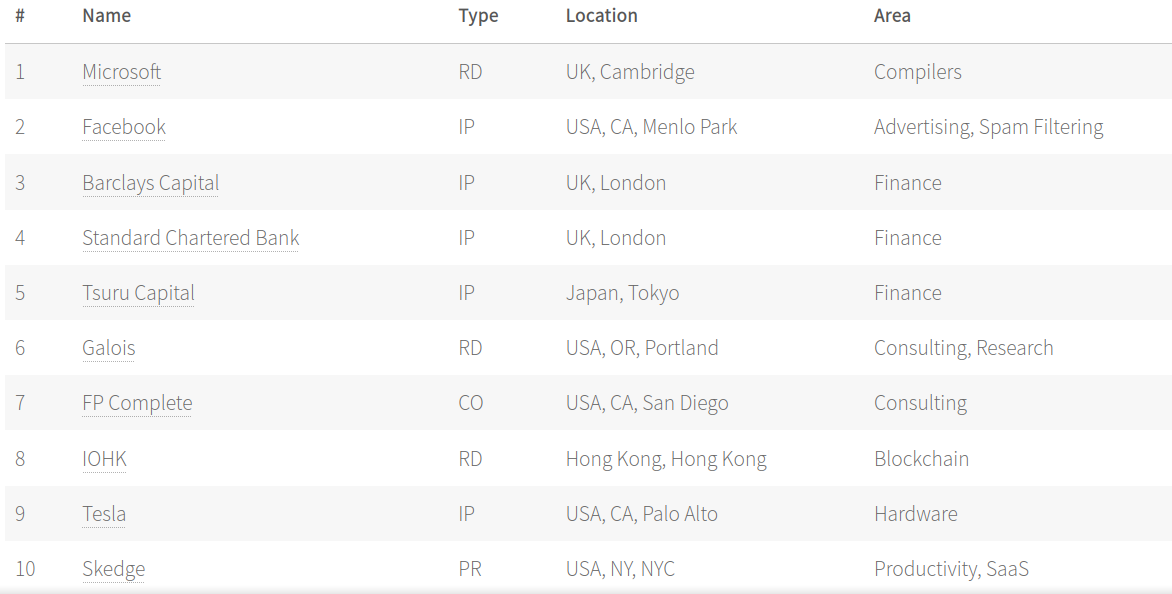
\includegraphics[height=.5\textheight]{Images/quiUtiliseHaskell.png}
\end{center}
\begin{block}{Exemples (\href{https://haskellcosm.com/}{lien})}
\begin{itemize}
\item Ryan Trinkle,  CEO de SKEDGE.ME témoigne -> (\href{https://www.youtube.com/watch?v=BveDrw9CwEg}{vidéo}):
\begin{itemize}
\item 80\% de réduction du code, \textasciitilde{}64x d'amélioration de la performance, suppression de bug importants.
\end{itemize}
\item Autre exemple chez Facebook (\href{https://www.youtube.com/watch?v=mlTO510zO78}{en video})
\end{itemize}
\end{block}
\end{frame}

\subsection{Mise en place}
\label{sec:orgeaea36d}
\begin{frame}[label={sec:org10b4ca0}]{Choisir un IDE}
\begin{block}{}
\only<1>{

\begin{center}
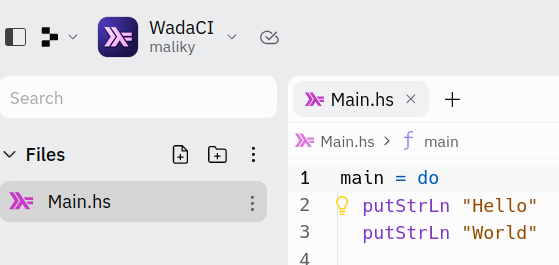
\includegraphics[height=.3\textheight]{Images/replit.png}
\end{center}

}

\only<2>{
\begin{center}
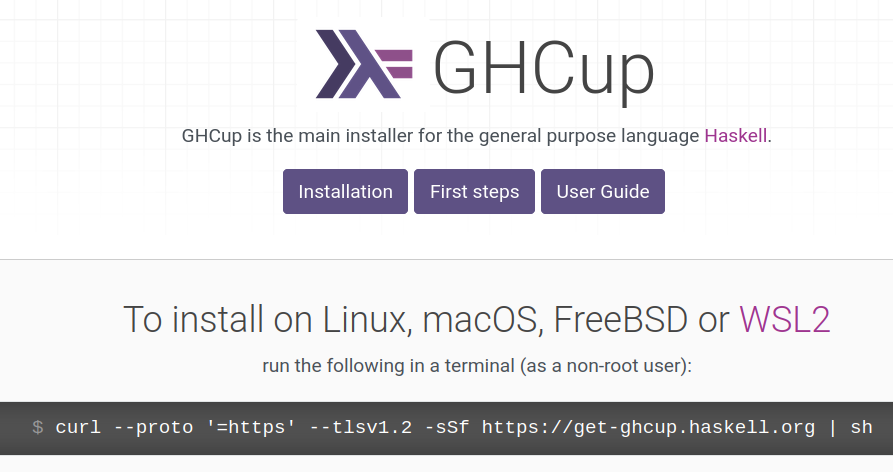
\includegraphics[height=.3\textheight]{Images/ghcup.png}
\end{center}

}

\only<3>{
\begin{center}

\includegraphics[height=.3\textheight]{Images/try_haskell.png}
\end{center}

}

\only<4>{
\begin{center}
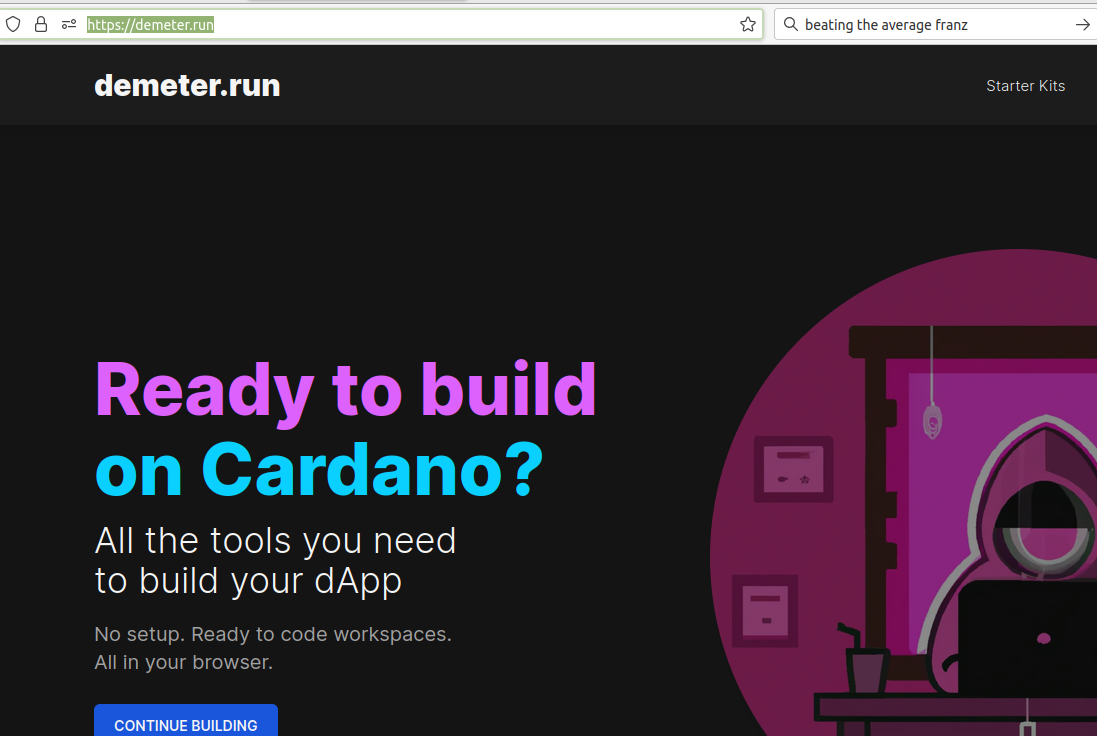
\includegraphics[height=.3\textheight]{Images/demeter.png}
\end{center}
}
\end{block}
\begin{block}{}
\begin{itemize}
\item <1->Replit IDE en ligne ->  \href{https://replit.com/join/ybqsuyuphr-maliky}{lien d'invitation}
\item <2->Installer ghci (\href{https://www.haskell.org/downloads/}{site officiel})
\begin{itemize}
\item Utiliser \href{https://www.haskell.org/ghcup/}{GHCUP} pour l'installation
\end{itemize}
\item <3-> \href{https://tryhaskell.org/\#step3}{Try Haskell}  : pour un essaye Haskell en ligne
\item <4-> \url{https://demeter.run/}
\end{itemize}
\end{block}
\end{frame}
\section{La pratique}
\label{sec:orgcbf5ace}
\subsection{Déroulement de l'atelier}
\label{sec:org28cb168}
\begin{frame}[label={sec:orge1c99c6}]{Déroulement de l'atelier}
\only<1>{
\begin{center}
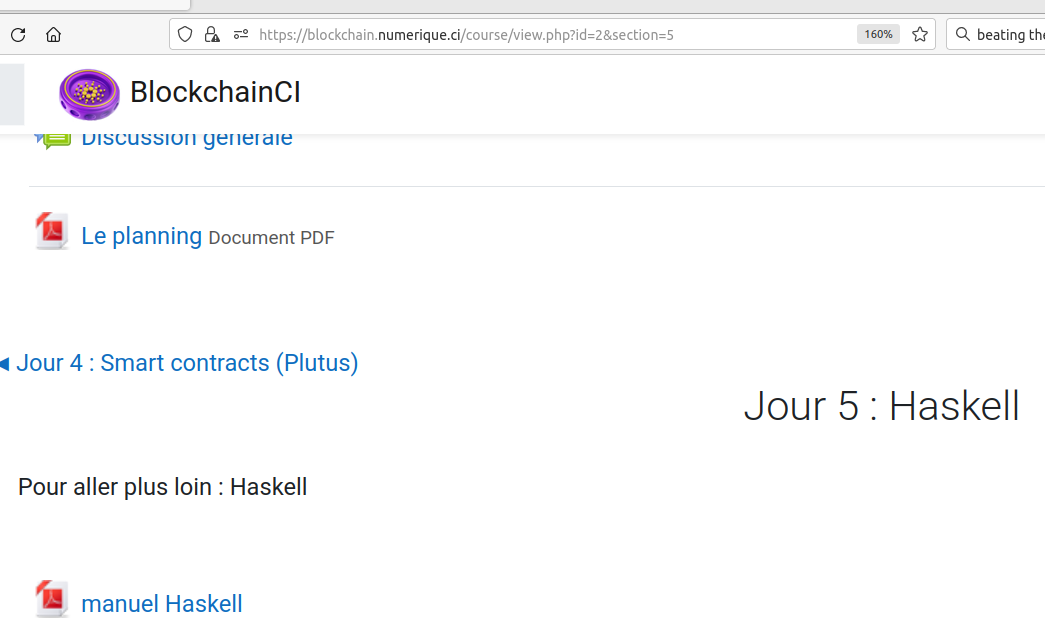
\includegraphics[height=.5\textheight]{Images/manuel_haskell.png}
\end{center}
}

\only<2>{
\begin{center}

\includegraphics[height=.5\textheight]{Images/manuel_contenu.png}
\end{center}
}
\only<3>{
\begin{center}
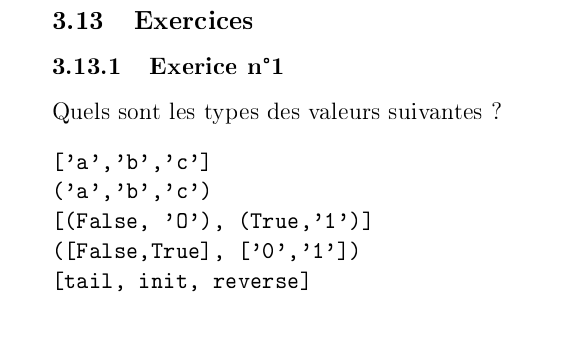
\includegraphics[height=.5\textheight]{Images/manuel_exercice.png}
\end{center}
}

\begin{itemize}
\item <1>Récupérer le manuel sur
\end{itemize}
\url{https://blockchain.numerique.ci/pluginfile.php/220/mod\_resource/content/1/manuel.pdf}
\begin{itemize}
\item <2> Suivre les contenus en reproduisant les codes dans votre IDE
\item <3> Résoudre les exerices et discuter leurs solutions avec vos camarades
\end{itemize}
\end{frame}
\subsection{Plan du cours}
\label{sec:orged82b31}
\begin{frame}[label={sec:orgbc5c1db}]{}
\begin{block}{Plan du cours}
\begin{itemize}
\item Que sont les 'Types' et les 'Classes de type'
\item Déclaration de fonctions
\item Listes en compréhension
\item Fonctions récursives
\item Fonctions de haut-niveau (higher-order)
\item Déclaration des Types et des Classes
\end{itemize}
\end{block}
\begin{block}{Le manuel (\textasciitilde{}40 pages)}
\end{block}
\end{frame}

\section{Ressoures et perspectives}
\label{sec:orgd0291f8}
\subsection{Ressources de formation}
\label{sec:org91b6df9}
\begin{frame}[label={sec:orgb81d234}]{Ressources de formation (\href{https://wiki.haskell.org/Haskell}{Haskell Wiki})}
\begin{block}<1->{Comprendre l'intérêt de la programmation fonctionnelle}
\begin{itemize}
\item \href{Ressources/beating\_average.pdf}{Faire mieux que la moyenne} (Paul Graham) (\href{https://franz.com/about/conferences/fds2001/presentations/pgtalk-rev2.pdf}{enligne})
\item \href{Ressources/why\_functionnal\_programming\_matter.pdf}{Pourquoi la programmation fonctionnelle est-elle importante ?} (John Hughes) (\href{https://www.cse.chalmers.se/\~rjmh/Papers/whyfp.pdf}{enligne})
\end{itemize}
\end{block}

\begin{block}<2->{Livres pour des études autonomes}
\begin{itemize}
\item \href{https://wiki.haskell.org/Books}{Liste de livres sur Haskell} (en)
\item \href{https://github.com/WADAlliance/Haskell\_Plutus\_Course}{Cours Haskell et de Plutus par WADA} (fr)
\item Livre populaire : \href{Ressources/learn\_you\_haskell\_for\_great\_good.pdf}{Apprendre Haskell vous fera du bien} (en \href{https://learnyouahaskell.github.io/chapters.html}{enligne})
\item Livre de grand qualité : \href{Ressources/Hutton\_G\_Programming\_in\_Haskell-Cambridge\_UP\_2018.pdf}{Programming in Haskell (2018, Hutton Graham)} (en, \href{https://www.cambridge.org/us/academic/subjects/computer-science/programming-languages-and-applied-logic/programming-haskell-2nd-edition}{enligne})
\end{itemize}
\end{block}
\begin{block}<3>{Cours en ligne gratuit}
\begin{itemize}
\item \href{https://www.futurelearn.com/courses/functional-programming-haskell}{Functional Programming Haskell} sur Futurlearn (en)
\end{itemize}
\end{block}
\end{frame}
\subsection{Perspectives}
\label{sec:orgc6b72f0}
\begin{frame}[label={sec:org6cc5f83}]{La suite\ldots{}  Création de l'association WADACI}
Donnera un cadre juridique pour :
\begin{itemize}
\item l'encadrement des prochaines formations (prochaine en mai)
\item les campagnes de communication et de sensibilisation grand publique
\item la réalisation de notre DAO
\end{itemize}
\begin{block}{Développement de projets crypto.}
\begin{columns}
\begin{column}{0.5\columnwidth}
\begin{block}{Idées pour le fond 10 ?}
\begin{itemize}
\item Transport
\item DAO 
\begin{itemize}
\item Administration d'écoles
\item co-propriétés locatives
\end{itemize}
\end{itemize}
\end{block}
\end{column}
\begin{column}{0.5\columnwidth}
\begin{block}{}
\begin{itemize}
\item traçabilité de titres fonciers (entre autres)
\item Observatoire des prix
\item Plateforme de financement de multi-media
\end{itemize}
\end{block}
\end{column}
\end{columns}
\end{block}
\end{frame}
\begin{frame}[label={sec:org02aac31}]{}
\begin{center}

\includegraphics[height=\textheight]{Images/merci_wadaci.png}
\end{center}
\end{frame}
\end{document}